\documentclass{llncs}
\usepackage[utf8]{inputenc}
\usepackage[T1]{fontenc}
\usepackage[final]{graphicx}
\usepackage{epstopdf}
\usepackage[labelsep=period]{caption}
\usepackage[hyphens]{url}
\usepackage{amssymb,amsmath,mathrsfs}
\usepackage[russian,english]{babel}
\usepackage{graphicx}
\usepackage{multicol}
\usepackage[ruled,vlined,linesnumbered,algosection,algo2e]{algorithm2e}
\usepackage{algorithm}
\usepackage[noend]{algorithmic}

\tolerance=1000
\hbadness=5000
\newcommand{\const}{\mathrm{const}}
\newcommand{\tsum}{\mathop{\textstyle\sum}\limits}
\newcommand{\tprod}{\mathop{\textstyle\prod}\limits}
\newcommand{\cov}{\mathop{\rm cov}\limits}
\newcommand{\Dir}{\mathop{\rm Dir}\nolimits}
\newcommand{\KL}{\mathop{\rm KL}\nolimits}
%\renewcommand{\geq}{\geqslant}
%\renewcommand{\leq}{\leqslant}
\newcommand{\eps}{\varepsilon}
\newcommand{\cond}{\mspace{3mu}{|}\mspace{3mu}}
\newcommand{\Loss}{\mathscr{L}}
\newcommand{\RR}{\mathbb{R}}
\newcommand{\cL}{\mathscr{L}}
\newcommand{\cP}{\mathscr{P}}
\SetKwFor{ForAll}{\textbf{for all}}{}{}

\begin{document}
%%Analysis of Images, Social Networks, and Texts
\title{
    BigARTM: Open Source Library for
    Regularized Multimodal %Online Parallel Distributed
    Topic Modeling of Large Collections
}
\author{
    Konstantin Vorontsov\inst{1,3}
    \and
    Oleksandr Frei\inst{2}
    \and
    Murat Apishev\inst{3}
    \and
    Peter Romov\inst{4}
}
\institute{
    Department of Intelligent Systems at Dorodnicyn Computing Centre of RAS,
    Moscow Institute of Physics and Technology,
    \email{voron@forecsys.ru}
    \and
    Schlumberger
    \email{...}
    \and
    Moscow State University,
    \email{...}
    \and
    Yandex
    \email{...}
}

\maketitle

\begin{abstract}
    BigARTM

\vspace{1em}
\textbf{Keywords:}
    probabilistic topic model,
    Probabilistic Latent Sematic Analysis,
    Latent Dirichlet Allocation,
    Additive Regularization of Topic Models,
    stochastic matrix factorization,
    EM-algorithm,
    BigARTM.
\end{abstract}

\section{Introduction}

Topic modeling is a~rapidly developing branch of statistical text analysis~\cite{blei12ptm}.
Topic model reveals a~hidden thematic structure of the text collection
and finds a~compressed representation of each document by~a~set of its topics.
Such models appear to be highly useful for many applications including
information retrieval for long-text queries, 
revealing research trends and research fronts,
classification, categorization, summarization and segmentation of texts.
More ideas, models and applications are outlined in the survey~\cite{daud10knowledge}.

From the statistical point of view, a~probabilistic topic model
defines each topic by a~multinomial distribution over words,
and then describes each document with a~multinomial distribution over topics.
From the optimizational point of view, 
topic modeling can be considered as a~special case 
of constrained approximate stochastic matrix factorization.  
Learning a~factorized representation of a~text collection
is an ill-posed problem, which has an infinite set of solutions.
Then a~regularization must be used 
to~impose problem-oriented restrictions 
and thus to choose a~more reasonable solution.

Hundreds of models adapted to different situations are described in the literature. 
For practitioners, most of them are too difficult to quickly 
understand, compare, combine and embed into applications.
Then there was a~common practice to use only the simplest models such as 
\emph{Probabilistic Latent Semantic Analysis}, PLSA~\cite{hofmann99plsi} and
\emph{Latent Dirichlet Allocation}, LDA~\cite{blei03latent}.
Some of the difficulties are rooted in Bayesian learning framework,
which is dominating approach in topic modeling. 
Bayesian inference of each kind of model is a~unique and laborious mathematical work,
which prevents the unification and the flexible manipulation of various topic models.
Until now, there was no freely available development tools 
to easily design, modify, select, and combine topic models.

In this paper we announce \textbf{the BigARTM open source project} for 
parallel distributed online topic modeling of large collections,
\texttt{http://bigartm.org}.
The theory of BigARTM is based on non-Bayesian multicriteria approach~--- 
\emph{Additive Regularization of Topic Models}, ARTM~\cite{voron14dan-eng}.
In~ARTM a~topic model is learned by maximizing the~weighted sum
of the log-likelihood and additional regularization criteria.
The optimization problem is solved by a~general regularized expectation-maximization (EM) algorithm,
in which any regularization criteria or their combination can be substituted.
Many known Bayesian topic models were revisited in terms of ARTM in~\cite{voron14aist,voron14mlj}.
Compared to the Bayesian approach,
ARTM makes topic models easier to design, infer, combine and explain,
thus reducing barriers to entry into topic modeling research field.

The rest of the paper is organized as follows.
In~section~\ref{sec:Multimodal} 
we~introduce a~multimodal topic model generalized for documents with multiple accompanying discrete metadata. 
In~section~\ref{sec:Online}
we~describe a~fast online algorithm~\cite{hoffman10online} generalized for any additively regularized topic models.
In~section~\ref{sec:BigARTM}
we~consider the parallel architecture and implementation details of BigARTM library.
In~section~\ref{sec:Experiments}
we~report some experiments on large datasets. 
In~section~\ref{sec:Conclusions} 
we~discuss advantages, limitations and open problems of BigARTM.


\section{Multimodal regularized topic model}
\label{sec:Multimodal}

%Matching Words and Pictures, MoM-LDA \cite{barnard03matching}
%\cite{virtanen12factorized}
%\cite{roller13multimodal}

Let
$D$ denote a finite set (collection) of texts and
$W^1$ denote a~finite set (vocabulary) of all terms from these texts.
Each term can be a~single word or a~key phrase.
%Each document ${d\in D}$ is a sequence of terms from the vocabulary~$W^1$.
Denote $n_{dw}$ the number of times the term~$w$ appears in the document~$d$.
A document can contain not only words, but also elements of other modalities, which we also call terms.
Each $j$-th modality is defined by the finite set (vocabulary) of its terms $W^j$, ${j=1,\dots,m}$.
Examples of not-word modalities are:
authors,
class or category labels,
date-time stamps,
references to or from other documents,
entities mentioned in texts,
objects found in the images illustrating texts,
users that read or downloaded documents,
advertising banners,
etc.

Following the ideas of Correspondence LDA~\cite{blei03modeling}
and Dependency LDA~\cite{rubin12statistical}
we introduce the topic model of each $j$-th modality:
\[
    p(w\cond d)
    = \sum_{t\in T} p(w\cond t)\: p(t\cond d)
    = \sum_{t\in T} \phi_{wt} \theta_{td},
    \quad 
    d\in D,\; w\in W^j,\; j=1,\dots,m.
\]

The model parameters 
$\phi_{wt}=p(w\cond t)$ and $\theta_{td}=p(t\cond d)$
form the matrixes 
$\Phi^j = \bigl( \phi_{wt} \bigr)_{W^j\times T}$ of \emph{term probabilities for the topics}, and
$\Theta = \bigl( \theta_{td} \bigr)_{T\times D}$ of \emph{topic probabilities for the documents}.
Matrixes $\Phi^j$, if stacked vertically, 
form ${W\!\!\times\!T}$-matrix~$\Phi$, 
where ${W=W^1\sqcup\cdots\sqcup W^m}$ is disjoint union of all modalities.
Matrices $\Phi^j$ and~$\Theta$ are \emph{stochastic},
that is, their columns $\phi^j_t$, $\theta_d$
are non-negative and normalized representing discrete distributions.
The number of topics~$|T|$ is usually assumed to be 
much smaller than~$|D|$ and some of~modalities~$|W^j|$.

To learn parameters $\Phi^j$, $\Theta$ from the multimodal text collection
we maximize the log-likelihood for $j$-th modality:
\[
    \cL_j (\Phi^j,\Theta) =
    \sum_{d\in D}\sum_{w\in W^j} n_{dw} \ln p(w\cond d)
    \to \max_{\Phi^j,\Theta},
\]
where
$n_{dw}$ is the number of occurrences of the term $w\in W^j$ in the document~$d$.
Note that topic distributions of documents $\Theta$ are common for all modalities.
Following the ARTM approach, 
we add a~regularization penalty term $R(\Phi,\Theta)$
and solve the constrained multicriteria optimization problem via scalarization:
\begin{gather}
\label{eq:multimodal}
    \sum_{j=1}^m \tau_j \cL_j (\Phi^j,\Theta) 
    + R(\Phi,\Theta)
    \to \max_{\Phi,\Theta};
\\\label{eq:multimodal:norm}
    \sum_{w\in W^j} \phi_{wt} = 1,~
    \phi_{wt}\geq 0;
    \qquad
    \sum_{t\in T} \theta_{td} = 1,~
    \theta_{td}\geq 0.
\end{gather}

\begin{theorem}
\label{th:multimodal}
    If the function $R(\Phi,\Theta)$ is continuously differentiable
    then the local maximum $(\Phi,\Theta)$
    of the problem~\eqref{eq:multimodal},~\eqref{eq:multimodal:norm}
    satisfies the system of equations
    with auxiliary variables $p_{tdw} = p(t\cond d,w)$:
    \begin{align*}
        p_{tdw} &\propto \phi_{wt}\theta_{td};
    \\
        \phi_{wt} &\propto
            \biggl(
                n_{wt} + \phi_{wt} \frac{\partial R}{\partial \phi_{wt}}
            \biggr)_{\!\!+};
        &
        n_{wt} &= \sum_{d\in D} n_{dw} p_{tdw};
    \\
        \theta_{td} &\propto
            \biggl(
                \sum_{j=1}^m \tau_j n^j_{td} + \theta_{td} \frac{\partial R}{\partial \theta_{td}}
            \biggr)_{\!\!+};
        &
        n^j_{td} &= \sum_{w\in W^j} n_{dw} p_{tdw}.
    \end{align*}
\end{theorem}

This statement follows from Karush--Kuhn--Tucker conditions.
The system of equations can be~solved by various numerical methods.
Particularly,
the simple-iteration method is equivalent to the EM algorithm,
which is typically used in~practice.
Note that with one modality (${m=1}$)
this theorem gives E-step and M-step equations of the regularized EM algorithm
in ARTM~\cite{voron14aist,voron14mlj}.
With no regularization (${R=0}$) it corresponds to 
probabilistic latent semantic analysis~\cite{hofmann99plsi}. 

\section{Online topic modeling}
\label{sec:Online}
%\cite{zhang13sparse}

Following the ideas of Online LDA \cite{hoffman10online}

\section{BigARTM architecture}
\label{sec:BigARTM}

\subsection{Algorithm}

\begin{algorithm}
\caption{Online EM-algorithm}
\label{fig:plsa_alg}
\begin{algorithmic}[1]
\STATE Initialize $\phi_{wt}$ for all $w \in W$ and $t \in T$;
\STATE $n_{wt} := 0$, $\tilde n_{wt} := 0$
\FORALL{batches $D_j$, j = 1,...,J}
    \STATE $\tilde n_{wt} := \tilde n_{wt} + ProcessBatch(D_j, \phi_{wt})$
    \IF{(synchronize)}
        \STATE $n_{wt} := Merge(n_{wt}, \tilde n_{dw})$;
        \STATE $r_{wt} := Regularize(n_{wt})$;
        %\STATE $n_t := \sum_{w \in W} max(0, n_{wt} + r_{wt})$;
        \STATE $\phi_{wt} := Normalize(n_{wt} + r_{wt})$;
        \STATE $\tilde n_{dw} := 0$;
    \ENDIF
\ENDFOR
\end{algorithmic}
\end{algorithm}

\begin{algorithm}
\caption{$ProcessBatch(D_j, \phi_{wt})$}
\label{fig:plsa_alg}
\begin{algorithmic}[1]
\REQUIRE Batch $D_j$, Matrix $\phi_{wt}$;
\ENSURE $n_{wt}$;
\STATE $n_{wt} := 0$ for all $w \in W$ and $t \in T$;
\FORALL{ $d \in D_j$}
	\STATE initialize $\theta_{td}$ for all $t \in T$;
	\REPEAT
		\STATE $Z_w := \sum_{t \in T} \phi_{wt} \theta_{td}$ for all $w \in d$;
		\STATE $\theta_{td} := \frac{1}{n_d} \sum_{w \in d} n_{dw} \phi_{wt} \theta_{td} / Z_w$
               for all $t \in T$;
	\UNTIL{$\theta_d$ converges};
	\STATE increment $\tilde n_{wt}$ by $n_{dw} \phi_{wt} \theta_{td} / Z_w$
           for all $w \in d$ and $t \in T$;
\ENDFOR
\end{algorithmic}
\end{algorithm}

\subsection{Concurrency}
BigARTM can utilize multiple CPU cores by processing several batches in parallel,
which follows the rule of expressing parallelism at the highest possible level.
A alternative would be to parallelize the $ProcessBatch(D_j, \phi_{wt})$ routine,
but keeping it simple has many obvious benefits --- single-threaded code is much easier to modify and optimize.

\begin{figure}[h!]
\begin{centering}
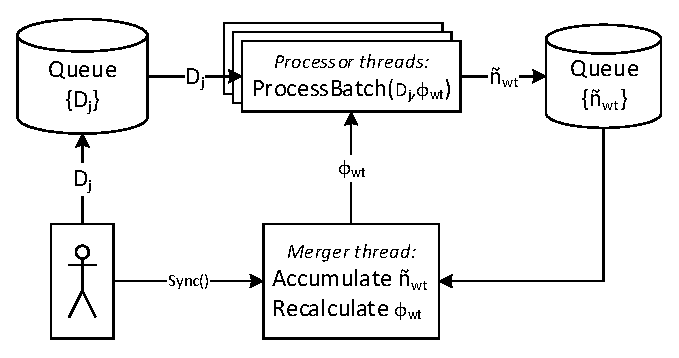
\includegraphics[height=48mm]{diagramm_artm_core.eps}
\caption{Diagram of key BigARTM components}
\label{fig:diagramm_artm_core}
\end{centering}
\end{figure}

Inputs and the outputs of $ProcessBatch$ routine are stored in two in-memory queues,
locked for push and pop operations with spin locks.
This approach does not add any noticeable synchronization overhead because
both queues only store smart pointers to the actual data objects,
so push and pop operations does not involve copying of real memory.

Smart pointers are also essential for handling of the $\phi_{wt}$ matrix.
This matrix is \emph{read} by all processors threads, and can be \emph{written} at any time by the merger thread.
To resolve this conflict we keep two copies of the $\phi_{wt}$ --- an \emph{active $\Phi$} and a \emph{background $\Phi$} matrices.
The active matrix is read-only, and is used by the processor threads.
The background matrix is being built in a background by the merger thread from $n_{wt}$ and $r_{wt}$ counters,
and once it is ready merger thread marks it as active.
Before processing a new batch the processor threads gets the current active matrix from the merger thread.
This object is passed via shared smart pointer to ensure that processor thread can keep ownership of the $\phi_{wt}$ matrix
until the batch is fully processed.

Having two copies of the $\Phi$ matrix is an obvious drawback of this solution.
An alternative would be to use atomic CPU instructions to read and write values of the $\Phi$ matrix.
Such operations are very efficient, but still come at a considerable synchronization cost
\footnote{http://stackoverflow.com/questions/2538070/atomic-operation-cost}.
Using them for all reads and writes of the $\Phi$ matrix would cause significant performance degradation for merger and processor threads.
Besides, an arbitrary overlap between reads and writes of the $\Phi$ matrix eliminates any possibility of producing a deterministic result.
The design with two copies of the $\Phi$ matrix give much more control over this
and in certain cases allows BigARTM to behave in a fully deterministic way.

The design with two $\Phi$ matrices only support a single merger thread,
and we believe it should cape with all $\hat n_{wt}$ updates coming from many threads.
This is a reasonable assumption because
$Merge$ routine takes only about $O(W * T)$ operations to execute, while
$ProcessBatch()$ takes $O(N_{nz} * T * I)$ operations,
where
$W$ is the size of the dictionary,
$N_{nz}$ is the number of non-zero entries in the batch,
$T$ is the number of topics,
and $I$ is the averate number of inner iterations in $ProcessBatch()$ routine.
$N_{nz} / W$ is typically 100 to 1000 (based on datasets in UCI Bag-Of-Words repository),
and $I$ is $10 \dots 20$, so the ratio safely exceeds the expected number of cores
(up to 32 physical CPU cores in modern workstations, and even 60 cores if we are talking about Intel Xeon Phi co-processors).

\subsection{Memory layout}

\subsection{Programming interface}

The core of BigARTM is written in C++, but we decided to wrap it into an ``extern C'' API.
This makes it very easy to consume BigARTM from almost any programming environment,
because there is always a way of calling ``extern C'' code
(ctypes module for Python, loadlibrary for Matlab, PInvoke for C\#, etc).








\section{Experiments}
\label{sec:Experiments}

\section{Conclusions}
\label{sec:Conclusions}

\bigskip
\subsubsection*{Acknowledgements.}
    The work was supported by~the Russian Foundation for Basic Research grants 14-07-00847, 14-07-00908,
    and by~Skolkovo Institute of Science and Technology (project 081-R).

%%%%%%%%%%%%%%%%%%%%%%%%%%%%%%%%%%%%%%%%%%%%%%%%%%%%%%%%%%%%%%%%%%%%%%%%%%%%
%\def\BibUrl#1.{\relax}
%\bibliographystyle{gost71sv}
\bibliographystyle{splncs}
\bibliography{MachLearn}
%%%%%%%%%%%%%%%%%%%%%%%%%%%%%%%%%%%%%%%%%%%%%%%%%%%%%%%%%%%%%%%%%%%%%%%%%%%%


\end{document}
